\chapter{Programa de trabajo}

El presente cronograma de actividades detalla la planificación estratégica para el desarrollo del proyecto de título, abarcando un periodo comprendido entre el 16 de marzo de 2026 y el 26 de agosto de 2026. La Carta Gantt integra, en una primera instancia, las etapas administrativas y de planificación exigidas por la facultad, seguidas del desarrollo técnico estructurado en torno a los cuatro objetivos específicos (OE): la caracterización aerodinámica (OE1), el modelado estructural (OE2), la evaluación de integridad normativa (OE3) y la planificación de manufactura CNC (OE4). Finalmente, se contempla el proceso transversal de redacción del informe final (OG) y el periodo de evaluación por comisión, culminando con la defensa del proyecto para asegurar el cumplimiento de todos los criterios de validación y los plazos institucionales establecidos.

\begin{sidewaysfigure}[htbp]
    \centering
    % El orden de trim es: izquierda inferior derecha superior
    % Los valores pueden ser en cm, mm o pt.
    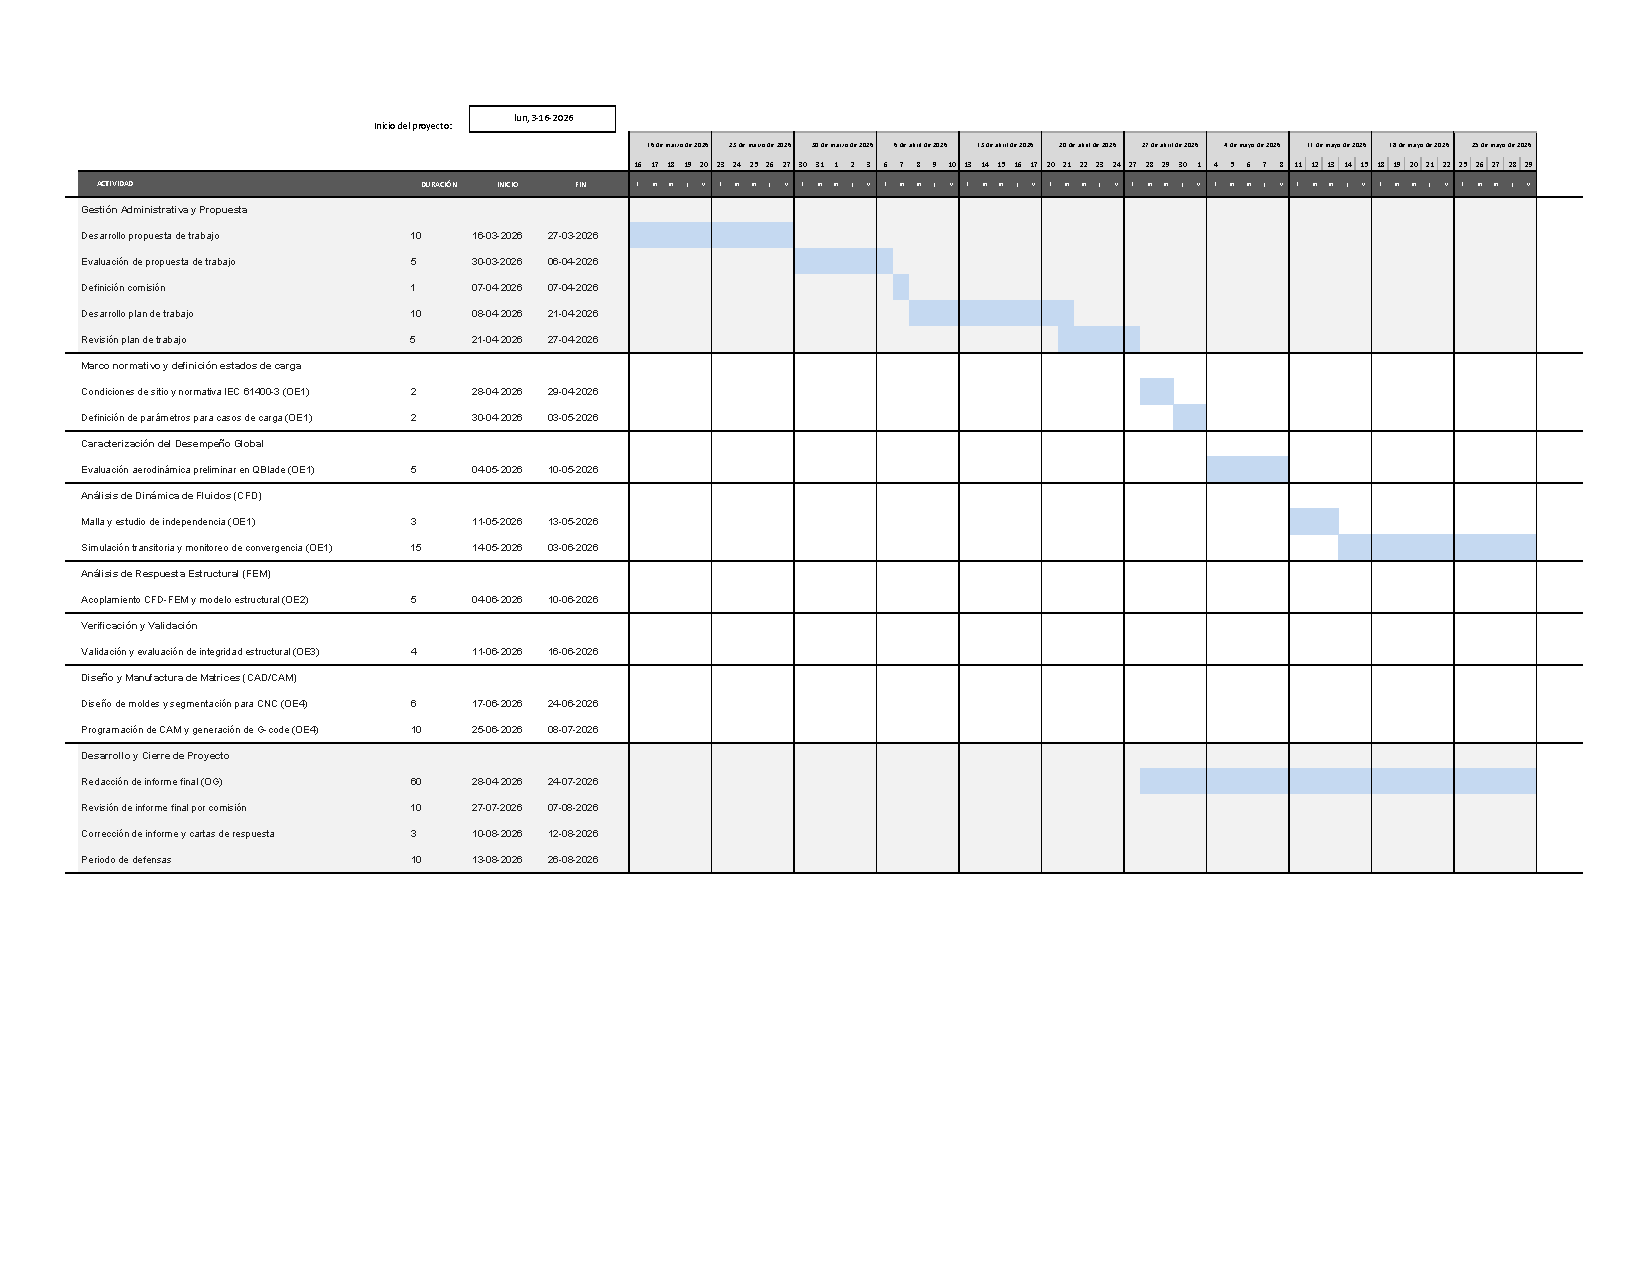
\includegraphics[trim={1cm 6cm 1,7cm 0cm}, clip, width=\textwidth]{Figuras/GANT1.pdf}
    \caption{Carta Gantt proyecto parte 1.}
\end{sidewaysfigure}

\begin{sidewaysfigure}[htbp]
    \centering
    % El orden de trim es: izquierda inferior derecha superior
    % Los valores pueden ser en cm, mm o pt.
    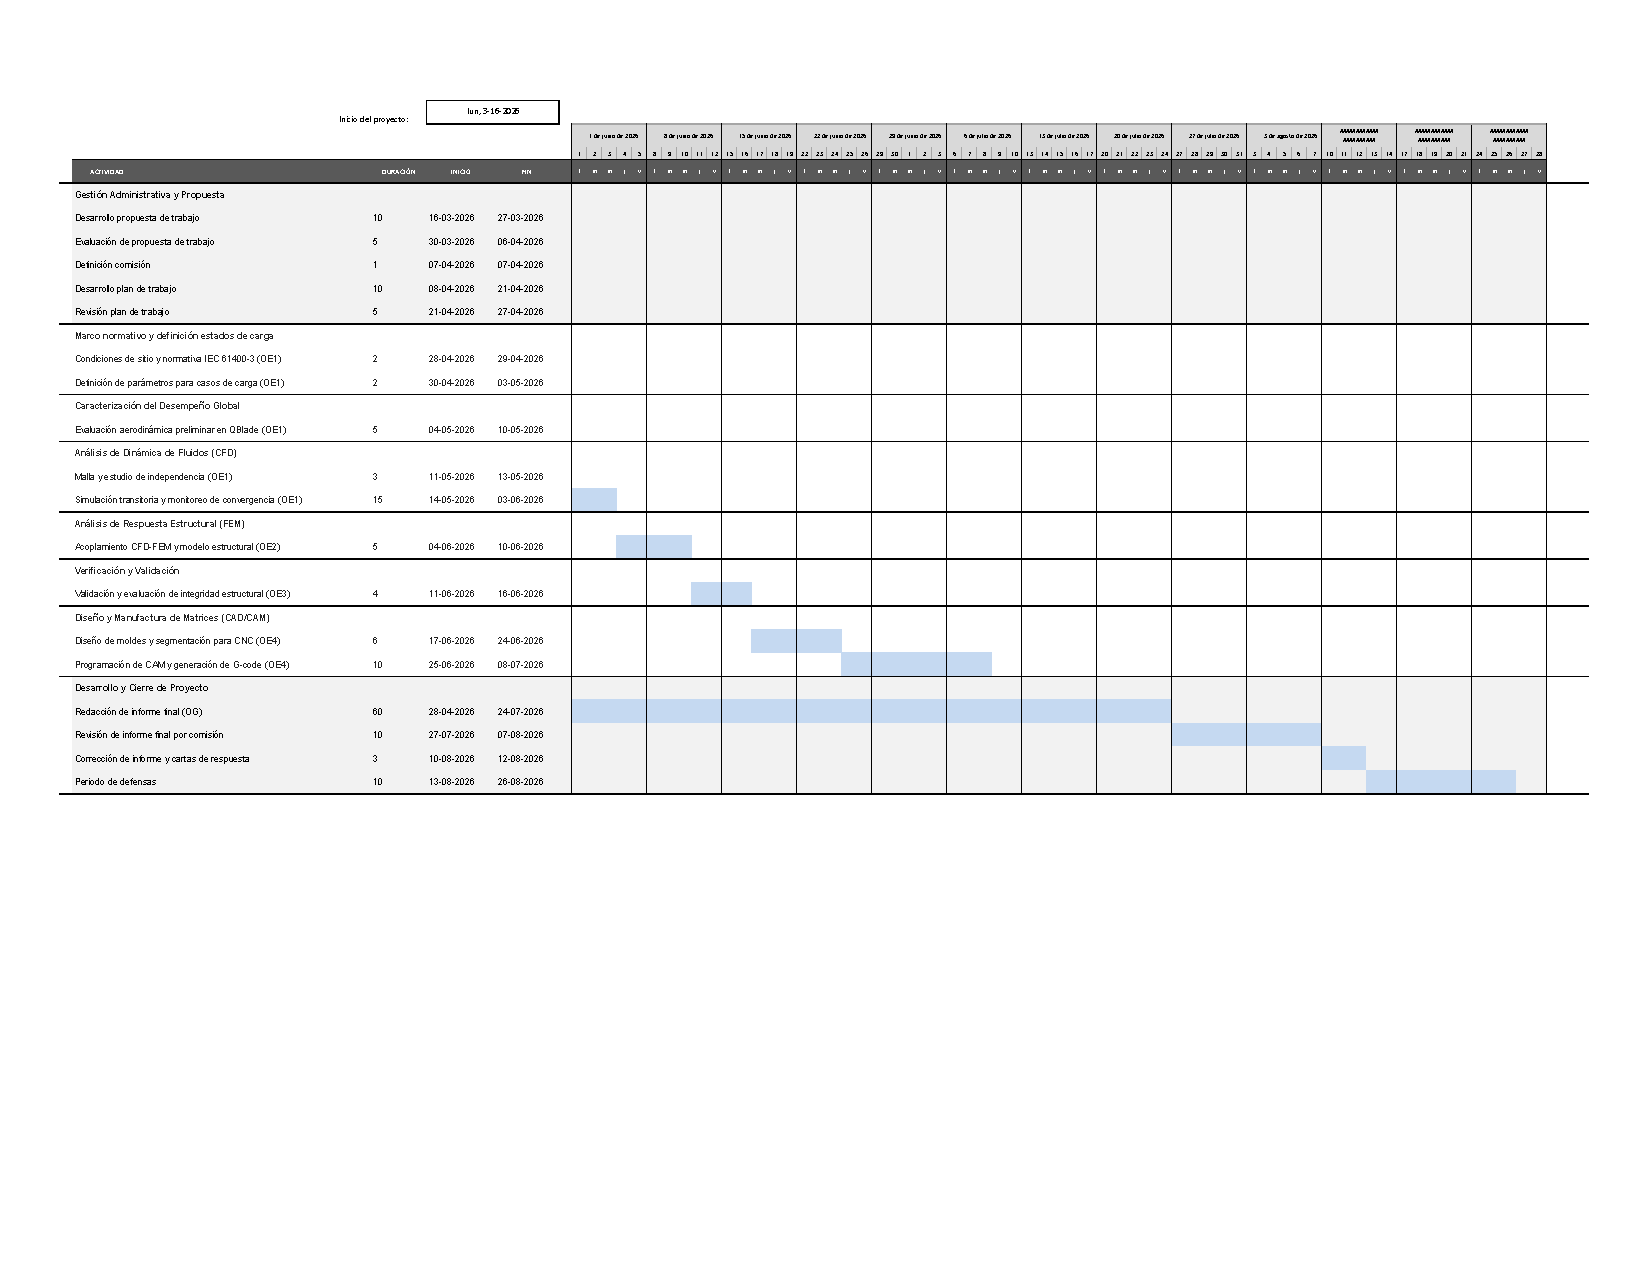
\includegraphics[trim={1cm 8cm 1,5cm 0cm}, clip, width=\textwidth]{Figuras/GANT2.pdf}
    \caption{Carta Gantt proyecto parte 2.}
\end{sidewaysfigure}